\section{Analysis}

    \subsection{Basic concepts}

    \begin{frame}{Skew in transmission lines}
        \begin{columns}
            \column{0.5\linewidth}
            \begin{itemize}
                \item<1-> Skew ($\Delta_T$) can be viewed as the difference in phase between two signals.
                \item<3-> If an interconnection's length is similar to that of the wave length ($\lambda$) of the signal, then a delay ($\Delta_{t_{TL}}$) will exist between A and B.
            \end{itemize}
            \vspace{0.4cm}
            \onslide<3->{\begin{equation*}
                \lambda = \frac{\nu_p}{f}
            \end{equation*}}
            \column{0.5\linewidth}
            \onslide<2->\begin{center}
                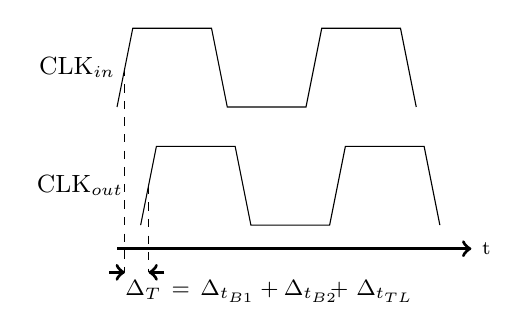
\begin{tikzpicture}
                    \draw (0,0) -- (0.2,1) -- (1.2,1) -- (1.4,0) -- (2.4,0) -- (2.6,1) -- (3.6,1) -- (3.8,0);   %CLK in
                    \draw (0.3,-1.5) -- (0.5,-0.5) -- (1.5,-0.5) -- (1.7,-1.5) -- (2.7,-1.5) -- (2.9,-0.5) -- (3.9,-0.5) -- (4.1,-1.5); %CLK out
                    \draw[dashed] (0.1,0.5) node[anchor=east]{\small{CLK$_{in}$}} -- (0.1,-2.1);  %dashed line
                    \draw[dashed] (0.4,-1) -- (0.4,-2.1);     %dashed line
                    \draw node[anchor=east] at (0.2,-1){\small{CLK$_{out}$}};
                    \draw[very thick, ->] (0,-1.8) -- (4.5,-1.8) node[anchor=west]{\scriptsize t};  %time arrow
                    \draw[->, very thick] (-0.1,-2.1) -- (0.1,-2.1);
                    \draw[->, very thick] (0.6,-2.1) -- (0.4,-2.1);
                    \draw node[anchor=north west, inner sep=0pt] at (0.1,-2.2) {\footnotesize $\Delta_T \, = \, \Delta_{t_{B1}} + \Delta_{t_{B2}}$};
                    \onslide<4->{\draw node[anchor=north west, inner sep=0pt] at (2.7,-2.2) {\footnotesize + \alert{$\Delta_{t_{TL}}$}};}
                \end{tikzpicture}
            \end{center}
            \vspace{0.5cm}
            \onslide<4->\begin{center}
                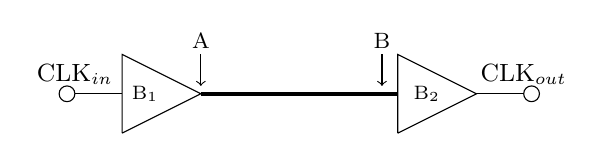
\begin{tikzpicture}
                    \draw (0,0) -- (0,1) -- (1,0.5) -- (0,0);   %buffer 1
                    \draw[ultra thick] (1, 0.5) -- (3.5,0.5);     %Transmission line
                    \draw (3.5,0) -- (3.5,1) -- (4.5,0.5) -- (3.5,0);   %buffer 2
                    \draw (-0.6,0.5) node[anchor=south]{\small CLK$_{in}$} -- (0,0.5) node[anchor=west]{\scriptsize B$_1$};
                    \draw (5.1,0.5) node[anchor=south]{\small CLK$_{out}$} -- (4.5,0.5) node[anchor=east, inner sep=13pt]{\scriptsize B$_2$};
                    \draw (-0.7,0.5) circle (0.1);  %terminal in
                    \draw (5.2,0.5) circle (0.1);   %terminal out
                    \draw[->] (1,1) node[anchor=south, inner sep=2pt]{\footnotesize A} -- (1,0.6);
                    \draw[->] (3.3,1) node[anchor=south, inner sep=2pt]{\footnotesize B} -- (3.3,0.6);
                \end{tikzpicture}
            \end{center}
        \end{columns}
    \end{frame}

    \begin{frame}{Skew correction}
        \begin{columns}
            \column{0.5\linewidth}
            \begin{itemize}
                \item<1-> How can we align CLK$_{out}$ with CLK$_{in}$ ?
                \item<2-> Since CLK$_{in}$ is periodic, an additional delay can be introduced at B$_2$ so as to make the total delay equal to once clock cycle (T$_{CLK}$).
            \end{itemize}
            \column{0.5\linewidth}
            \onslide<2->\begin{center}
                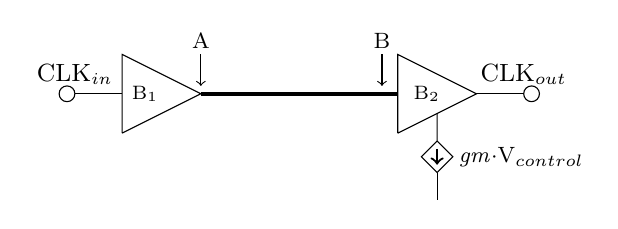
\begin{tikzpicture}
                    \draw (0,0) -- (0,1) -- (1,0.5) -- (0,0);   %buffer 1
                    \draw[ultra thick] (1, 0.5) -- (3.5,0.5);     %Transmission line
                    \draw (3.5,0) -- (3.5,1) -- (4.5,0.5) -- (3.5,0);   %buffer 2
                    \draw (4,0.25) -- (4,-0.1) -- (3.8,-0.3) --(4,-0.5) -- (4.2,-0.3) node[anchor=west, inner sep=2pt] {\footnotesize \textit{gm}$\cdot$\alert{V$_{control}$}} -- (4,-0.1);
                    \draw (4,-0.5) -- (4,-0.85);
                    \draw[->, thick] (4,-0.2) -- (4,-0.4);
                    \draw (-0.6,0.5) node[anchor=south]{\small CLK$_{in}$} -- (0,0.5) node[anchor=west]{\scriptsize B$_1$};
                    \draw (5.1,0.5) node[anchor=south]{\small CLK$_{out}$} -- (4.5,0.5) node[anchor=east, inner sep=13pt]{\scriptsize B$_2$};
                    \draw (-0.7,0.5) circle (0.1);  %terminal in
                    \draw (5.2,0.5) circle (0.1);   %terminal out
                    \draw[->] (1,1) node[anchor=south, inner sep=2pt]{\footnotesize A} -- (1,0.6);
                    \draw[->] (3.3,1) node[anchor=south, inner sep=2pt]{\footnotesize B} -- (3.3,0.6);
                \end{tikzpicture}
            \end{center}
            \vspace{0.5cm}
            \onslide<3->\begin{center}
                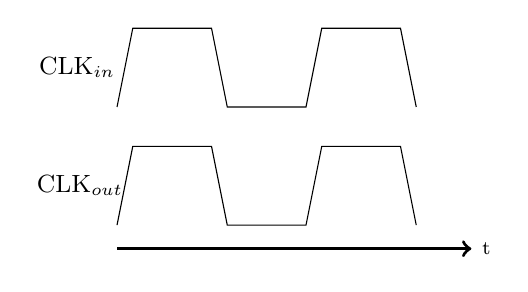
\begin{tikzpicture}
                    \draw (0,0) -- (0.2,1) -- (1.2,1) -- (1.4,0) -- (2.4,0) -- (2.6,1) -- (3.6,1) -- (3.8,0);   %CLK in
                    \draw (0,-1.5) -- (0.2,-0.5) -- (1.2,-0.5) -- (1.4,-1.5) -- (2.4,-1.5) -- (2.6,-0.5) -- (3.6,-0.5) -- (3.8,-1.5); %CLK out
                    \draw node[anchor=east] at (0.1,0.5) {\small CLK$_{in}$};
                    \draw node[anchor=east] at (0.2,-1) {\small CLK$_{out}$};
                    \draw[very thick, ->] (0,-1.8) -- (4.5,-1.8) node[anchor=west]{\scriptsize t};  %time arrow
                \end{tikzpicture}
            \end{center}
        \end{columns}
    \end{frame}

    \subsection{Blocks}

    \begin{frame}{DLL as a black box}
        
        \begin{columns}
            \column{0.5\linewidth}
            \begin{itemize}
                \item<1-> The DLL can be modeled as a box that takes in a control voltage and CLK$_{in}$, and outputs CLK$_{out}$ in phase with the reference.
            \end{itemize}
            \column{0.5\linewidth}
            \onslide<2->\begin{center}
                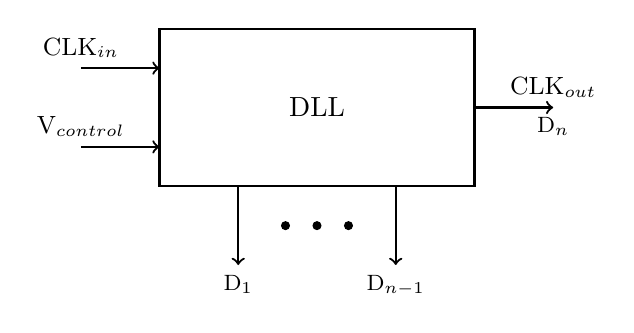
\begin{tikzpicture}
                    \draw[thick] (0,0) rectangle (4,2);
                    \draw node at (2,1) {DLL};
                    \draw[->, thick] (-1,1.5) node[anchor=south] {\small CLK$_{in}$} -- (0,1.5);
                    \draw[->, thick] (-1,0.5) node[anchor=south] {\small V$_{control}$} -- (0,0.5);
                    \draw[->, thick] (4,1) -- (5,1) node[anchor=south] {\small CLK$_{out}$};
                    \onslide<4->{\draw node[anchor=north] at (5,1) {\footnotesize D$_n$};}
                    \onslide<4->{\draw[->, thick] (1,0) -- (1,-1) node[anchor=north] {\footnotesize D$_1$};}
                    \onslide<4->{\filldraw (1.6,-0.5) circle (0.05);}
                    \onslide<4->{\filldraw (2,-0.5) circle (0.05);}
                    \onslide<4->{\filldraw (2.4,-0.5) circle (0.05);}
                    \onslide<4->{\draw[->, thick] (3,0) -- (3,-1) node[anchor=north] {\footnotesize D$_{n-1}$};}
                \end{tikzpicture}
            \end{center}
        \end{columns}
        \vspace{1cm}
        \begin{block}{Why use a DLL at all?}<3->
            \onslide<4->Because of $\Delta_{t_{TL}}$ and the DLL's ability to generate multiple phases.
        \end{block}
    \end{frame}

    \begin{frame}{DLL block diagram}
        DLL block diagram
    \end{frame}

    \subsection{Schematics}

    \begin{frame}{PFD}
        PFD schematic
    \end{frame}